\documentclass[12pt]{article}
\usepackage[margin=0.65in]{geometry} %to adjust page margins
%What is visible in tableofcontents? 
%0->part 1->section, 2->subsection, 3-> subsubsection 4->paragraph 5-> subparagraph
\setcounter{tocdepth}{4}
%To number until {No}
\setcounter{secnumdepth}{4}

%\usepackage{amsmath}
\usepackage[cm-default]{fontspec}
\setmainfont{Times New Roman}

%Greek hyphenation
\usepackage{xgreek}

\usepackage{graphicx}
\usepackage{listings}
%TO keep pictures and tables exactly where they are {H}
\usepackage{float}

\usepackage{caption}
\usepackage{mathtools}%text above arrows
%\usepackage{framed}
\usepackage{hyperref}%for links in refs
%\usepackage{placeins}%FloatBarrier (y)
\usepackage{fancyhdr}%page style
%\usepackage{color}

%About theorems, lemmas etc
\newtheorem{mydef}{Ορισμός}
\newtheorem{mylem}{Λήμμα}
\newtheorem{mytheorem}{Θεώρημα}
\newtheorem{theorem}{Theorem}[section]
\newtheorem{corollary}{Corollary}[theorem]
\newtheorem{lemma}[theorem]{Lemma}

%For algorithms
\usepackage[ruled,linesnumbered]{algorithm2e}

%For nice highlighting in code files
\usepackage[usenames,dvipsnames,svgnames,table]{xcolor}
\usepackage{color}
\definecolor{vimyellow}{rgb}{0.4,0.4,0}
\definecolor{vimblue}{rgb}{0,0,0.6}
\definecolor{mymauve}{rgb}{0.58,0,0.82}
\lstset{breaklines=true, xleftmargin=\parindent, language=C, keywordstyle=\color{vimyellow}, commentstyle=\color{vimblue},stringstyle=\color{red}, numbers=left, tabsize=3 }

%For reals set R, Q, 
\usepackage{amsfonts}

%\usepackage[•]{•}8x}{inputnc}

%2C "εικονα #" αντί για "Figure #"
\renewcommand{\figurename}{Εικόνα}
%2C "Πίνακας #" αντί για "Table #"
\renewcommand{\tablename}{Πίνακας}

%For more readable fractions
\newcommand\ddfrac[2]{\frac{\displaystyle #1}{\displaystyle #2}}

%Do not display date
\date{}
\pagestyle{fancy}
\lhead{Νευρωνικά Δίκτυα και Ευφυή Υπολογιστικά Συστήματα}
\rhead{Άσκηση 1}
%\pagenumbering{gobble}
\begin{document}
\begin{titlepage}
\date{}
\begin{center}

\includegraphics[width=0.2\textwidth]{logo_ntua.jpg}\\

\textsc{\LARGE Σχολή Ηλεκτρολόγων Μηχανικών και Μηχανικών Υπολογιστών Ε.Μ.Π.}\\[1.5cm]
\LARGE
ΝΕΥΡΩΝΙΚΑ ΔΙΚΤΥΑ ΚΑΙ ΕΥΦΥΗ ΥΠΟΛΟΓΙΣΤΙΚΑ ΣΥΣΤΗΜΑΤΑ\\
2016-2017\\
\vfill
ΕΡΓΑΣΤΗΡΙΑΚΗ ΑΣΚΗΣΗ 1\\
\vfill
Ευαγγελία-Σοφία Γεργατσούλη\\
ΑΜ: 03112064\\
Νικηφόρος Μανδηλαράς\\
ΑΜ: 03112012\\
Εξάμηνο:9ο\\
\vfill
\end{center}
\end{titlepage}
%\tableofcontents %sections should me umbered to be included here
\newpage

\section*{Ερώτημα 1 - Προεπεξεργασία των δεδομένων}
	Αρχικά γίνεται μια προεπεξεργασία των δεδομένων για να γίνει σωστότερα η εκπαίδευση του δικτύου μας. Πιο συγκεκριμένα, θέλουμε να κρατήσουμε ίδιο αριθμό δειγμάτων ανα κατηγορία για να γίνει ίση εκπαίδευση σε κάθε περίπτωση κατηγορίας. Επιπλέον χρειαζόμαστε κανονικοποίηση των δεδομένων ώστε να επιταχύνεται η διαδικασία μάθησης στον αλγόριθμο back propagation και να αποφεύγονται οι περιπτώσεις "ταλάντωσης" κατα την διάδοση των αλλαγών στα βάρη. Για την επεξεργασία ακολουθήσαμε τα εξής βήματα:
	\begin{enumerate}
		\item Αφού φορτώθηκαν τα δεδομένα εισόδου, βρήκαμε με την εντολή sum πόσα τμήματα εικόνας περιέχει κάθε κατηγορία το οποίο είναι απλώς το άθροισμα της κάθε γραμμής του πίνακα TrainDataTargets για κάθε μια από τις 5 διαφορετικές γραμμές-κατηγορίες. Το αποτέλεσμα φαίνεται στο αριστερό bar διαγραμμα της εικόνας \ref{fig:2.1-parts-per-cat}. Όπως φαίνεται, δεν υπάρχει ο ίδιος αριθμός τμημάτων εικόνας για κάθε κατηγορία.
		\item Στη συνέχεια, για την διευκόλυνση της εκπαίδευσης του δικτύου, περνάμε τα δεδομένα απο επεξεργασία με τις removeconstantrows, mapstd και processpca. Η πρώτη αφαιρεί από τον πίνακα τις γραμμές που έχουν σταθερή τιμή (οι οποίες ουσιαστικά είναι άχρηστες). Η mapstd κανονικοποιεί τα δεδομένα, έτσι ώστε κάθε γραμμή του πίνακα να έχει μέση τιμή 0 και variance 1 και η processpca  κρατάει έναν μικρότερο αριθμό γραμμών του πίνακα σε περίπου 20 χωρίς να χάσει σημαντική πληροφορία (για να γίνει αυτό δίνουμε τιμή 0.01 στην παράμετρο maxfrac).
	\end{enumerate}
	Τελικά μετά την επεξεργασία παίρνουμε το δεξί bar διαγραμμα της εικόνας \ref{fig:2.1-parts-per-cat}. Η συνάρτηση γι αυτό το κομμάτι είναι η \textit{preproc.m}.
	
		\begin{figure}[H]
	 		\centering
			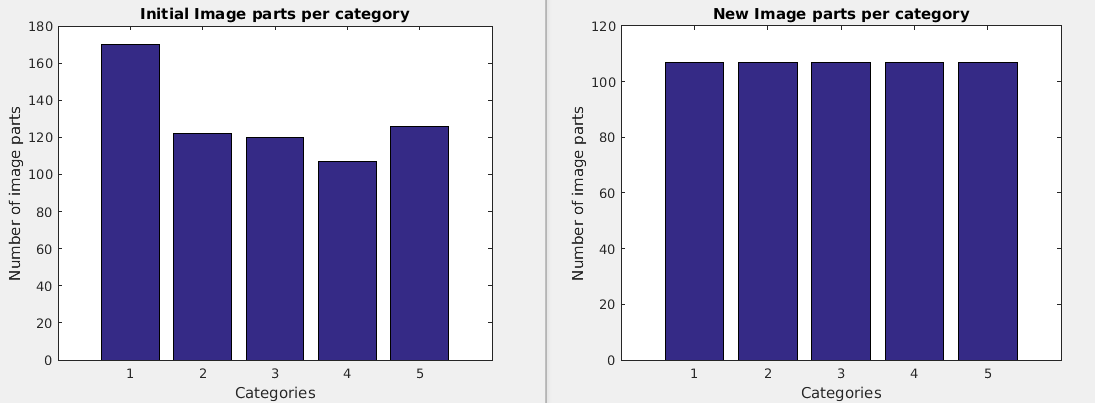
\includegraphics[width=0.9\textwidth]{fakelos/parts-per-cat.png}
			\caption{} 	  
			\label{fig:2.1-parts-per-cat}
		\end{figure}

\section*{Ερώτημα 2 - Διαφορετικές συναρτήσεις εκπαίδευσης και αριθμός επιπέδων και νευρώνων}
Καθώς η αρχικοποίηση γίνεται τυχαία όταν γίνεται η προεπεξεργασία των δεδομένων, κάθε φορά που φτιάχνουμε ένα νεο νευρωνικό δίκτυο, και μετράμε την απόδοση του δε θα παίρνουμε πάντα το ίδιο αποτέλεσμα. Μετά απο μετρήσεις σε πολλά διαφορετικά "τρεξίματα" καταλήξαμε στο ότι η καλύτερη συνάρτηση εκπαίδευσης είναι η trainlm (η οποία υλοποιεί τον αλγόριθμο Levenberg-Marquardt), καθως είχε στην πλειοψηφία των περιπτώσεων καλύτερη απόδοση από όλες τις άλλες για κάθε συνδυασμό νευρώνων 1ου και 2ου επιπέδου. Η αμέσως επόμενη καλύτερη ήταν η traingdx και σπανίως έβγαινε η traingda. Η traingd είχε πάντα τη χειρότερη απόδοση απ' όλες. Στις εικόνες \ref{fig:2.NN-lvls0}-\ref{fig:2.NN-lvls30} φαίνεται η απόδοση για κάθε συνάρτηση εκπαίδευσης και για κάθε συνδυασμό νευρώνων 1ου και 2ου επιπέδου. \\
\noindent
Αρχικά παρατηρούμε ότι περισσότεροι νευρώνες δεν συνεπάγονται και καλύτερη απόδοση καθώς όσο πιο πολύ "εξειδικεύεται" το δίκτυο υπάρχει ο κίνδυνος να μην μπορεί να γενικεύσει και απλώς να "θυμάται" τα δεδομένα εκπαίδευσης, δηλαδή να έχουμε overfitting.\\
Τέλος παρατηρήθηκε ότι τα καλύτερα αποτελέσματα τα παίρνουμε για λίγους εως καθόλου νευρώνες στο 2ο επίπεδο και μέτριο αριθμό νευρώνων 1ου επιπέδου. Συνγεκριμένα ο συνδυασμός 30 νευρώνες 1ου επιπέδου και 0 νευρώνες στο 2ο επίπεδο βγήκε νικητής τις περισσότερες φορές, άρα θα χρησιμοποιήσουμε αυτόν στα επόμενα ερωτήματα. Να σημειωθεί επίσης ότι η trainlm ήταν και αυτή που έτρεχε γρηγορότερα από τις υπόλοιπες, με πιο αργή την traingdx. Η συνάρτηση γι αυτό το κομμάτι είναι η \textit{myTrain.m}.

		\begin{figure}[H]
	 		\centering
			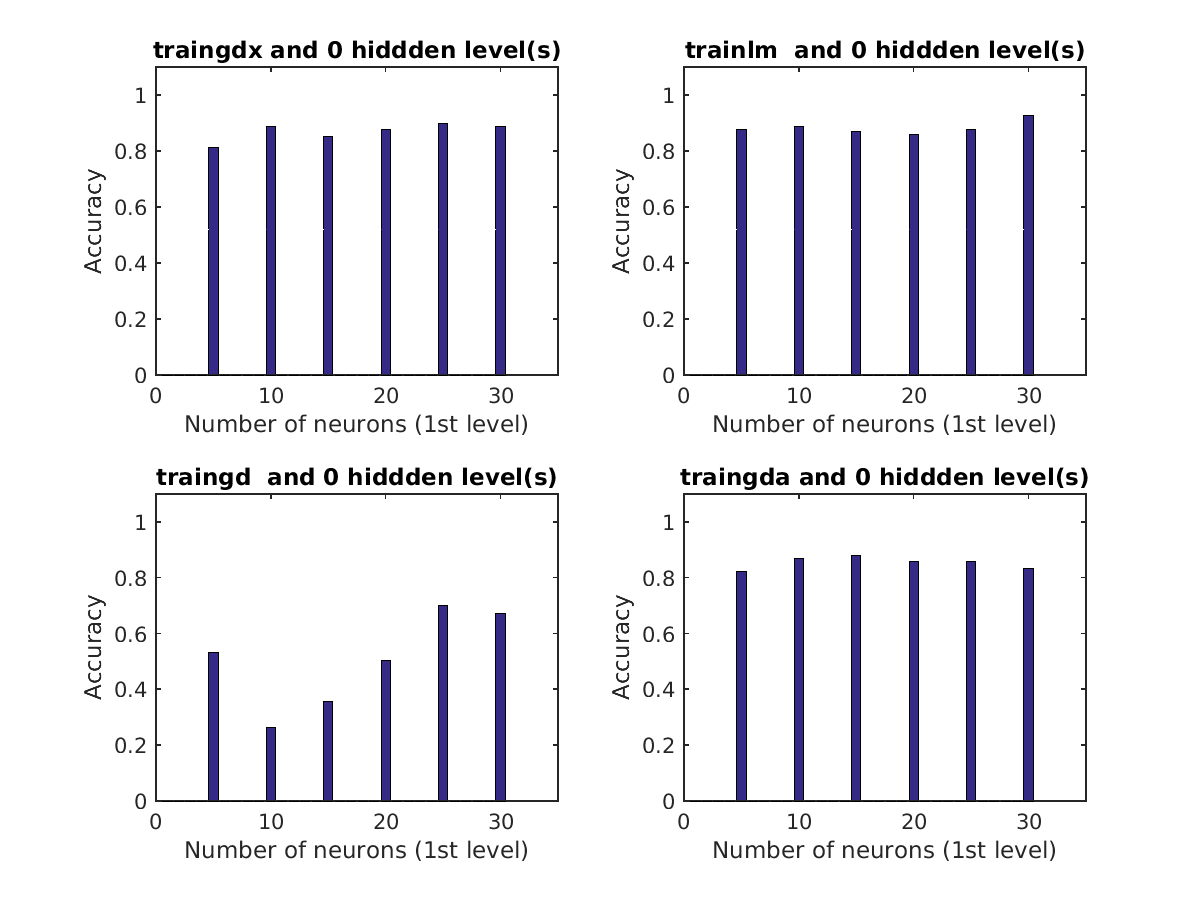
\includegraphics[width=0.8\textwidth]{fakelos/NNlvls-0.png}
			\caption{Απόδοση χωρίς 2ο κρυφό επίπεδο} 	  
			\label{fig:2.NN-lvls0}
		\end{figure}

		\begin{figure}[H]
	 		\centering
			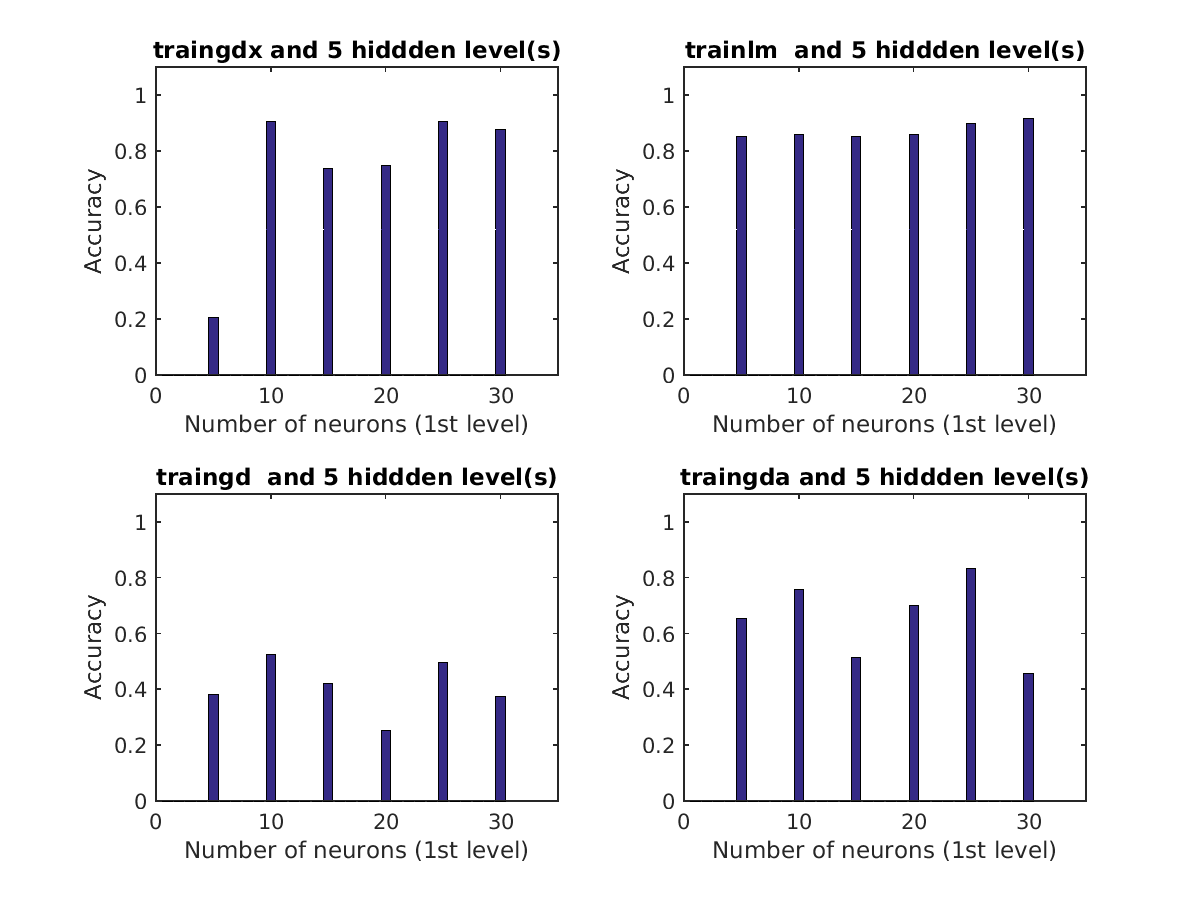
\includegraphics[width=0.8\textwidth]{fakelos/NNlvls-5.png}
			\caption{Απόδοση με 5 νευρώνες στο 2ο κρυφό επίπεδο} 	  
			\label{fig:2.NN-lvls5}
		\end{figure}
		
		\begin{figure}[H]
	 		\centering
			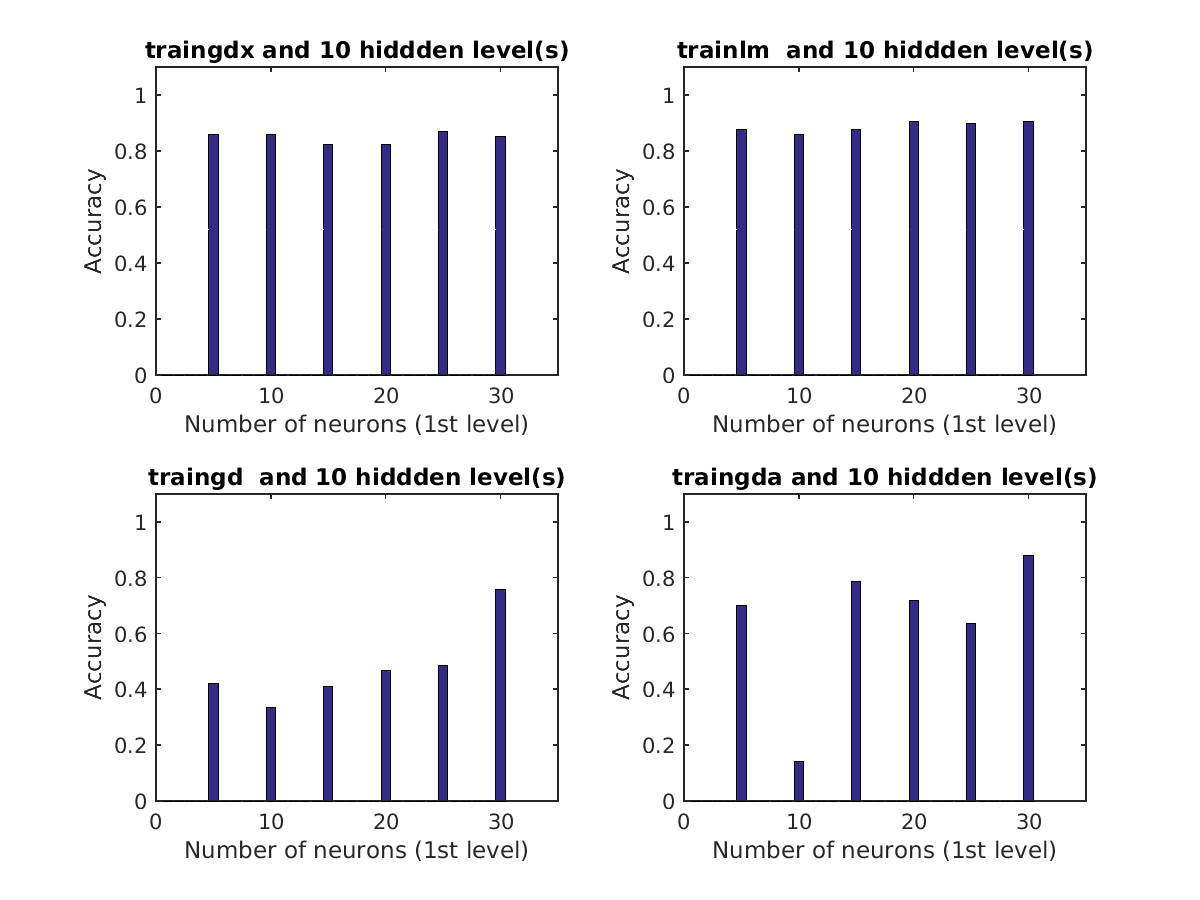
\includegraphics[width=0.8\textwidth]{fakelos/NNlvls-10.png}
			\caption{Απόδοση με 10 νευρώνες στο 2ο κρυφό επίπεδο} 	  
			\label{fig:2.NN-lvls10}
		\end{figure}

		\begin{figure}[H]
	 		\centering
			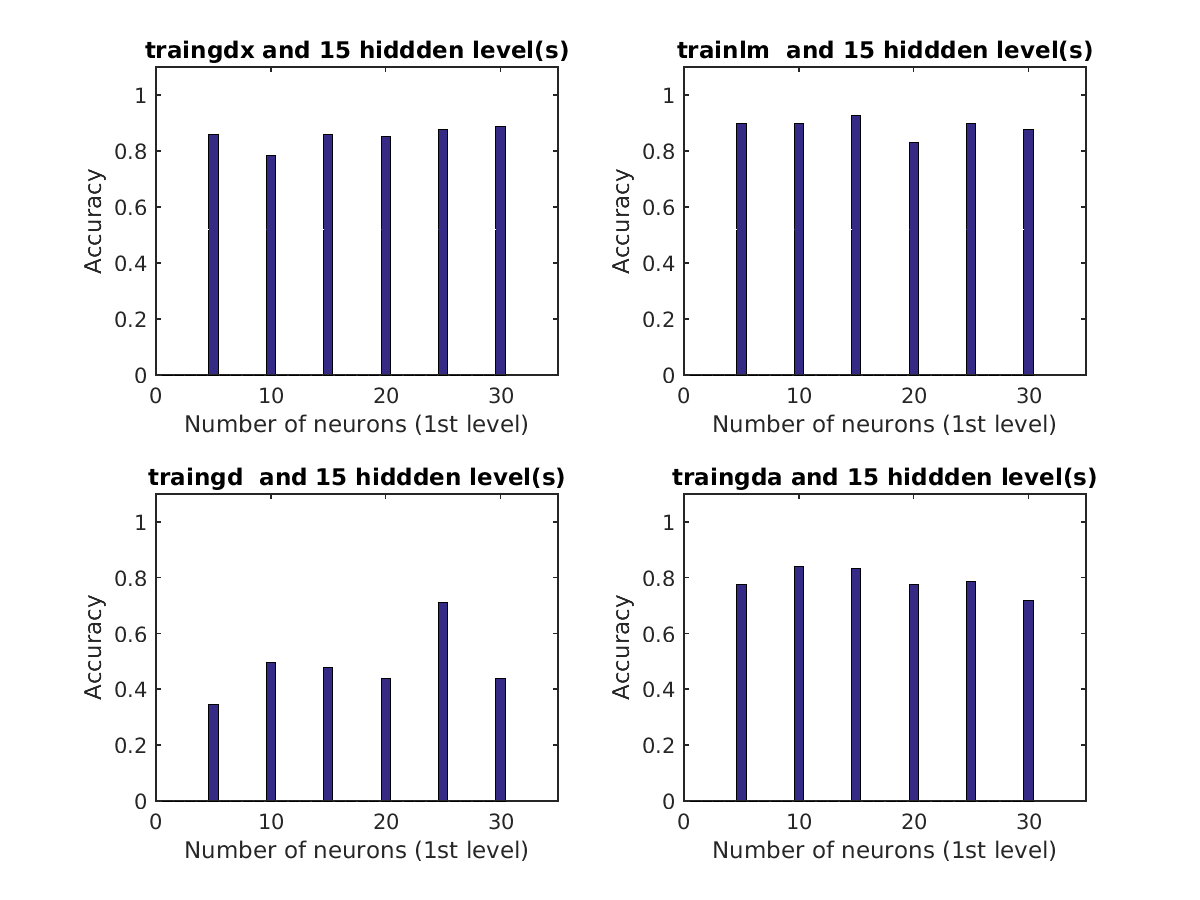
\includegraphics[width=0.8\textwidth]{fakelos/NNlvls-15.png}
			\caption{Απόδοση με 15 νευρώνες στο 2ο κρυφό επίπεδο} 	  
			\label{fig:2.NN-lvls15}
		\end{figure}

		\begin{figure}[H]
	 		\centering
			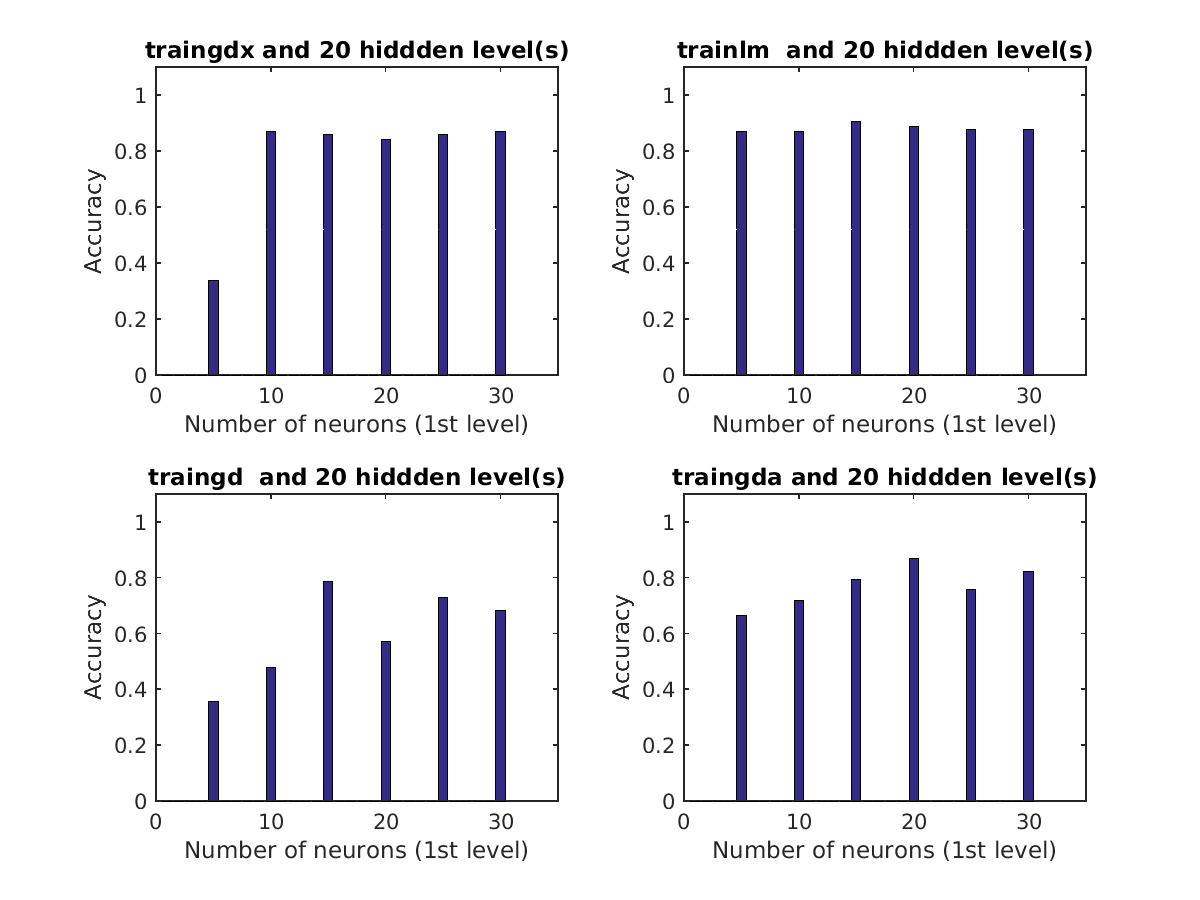
\includegraphics[width=0.8\textwidth]{fakelos/NNlvls-20.png}
			\caption{Απόδοση με 20 νευρώνες στο 2ο κρυφό επίπεδο} 	  
			\label{fig:2.NN-lvls20}
		\end{figure}
		
		\begin{figure}[H]
	 		\centering
			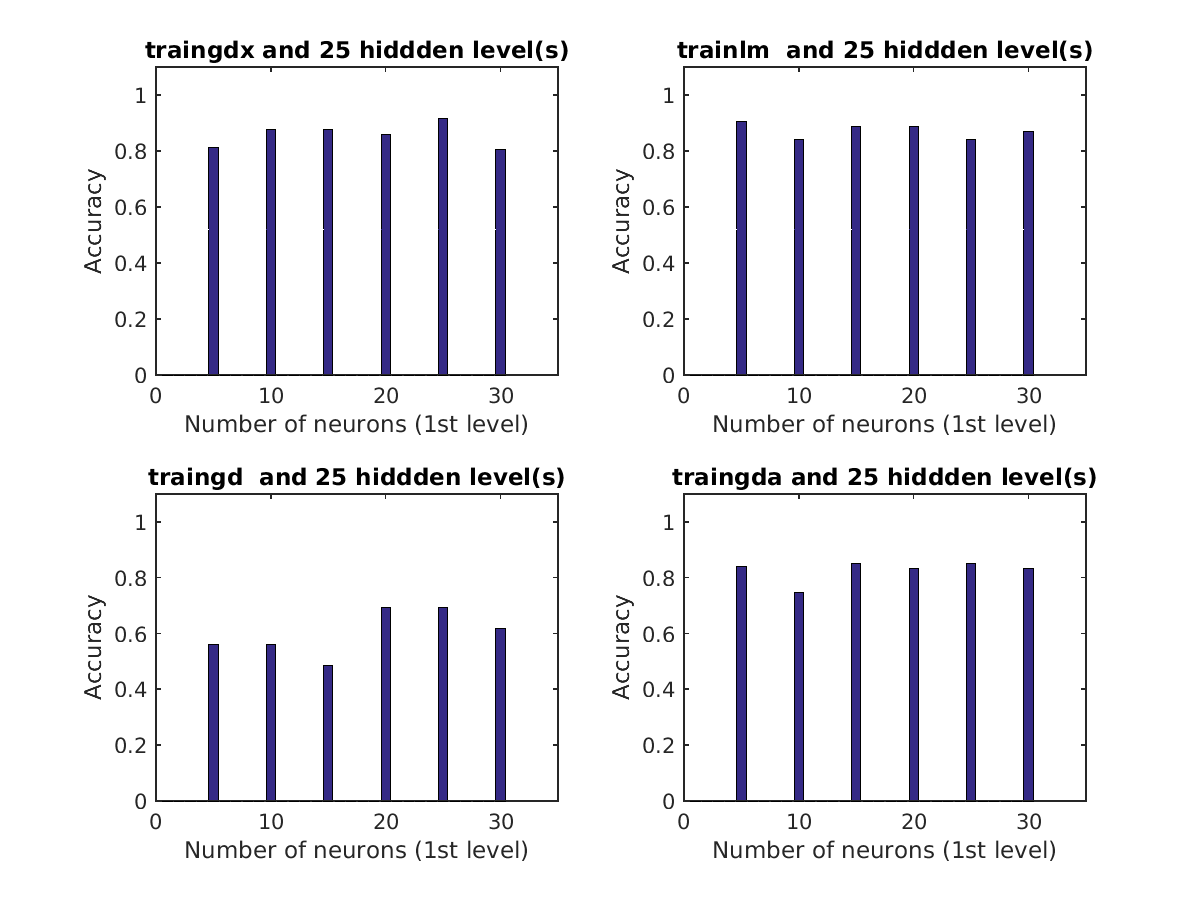
\includegraphics[width=0.8\textwidth]{fakelos/NNlvls-25.png}
			\caption{Απόδοση με 25 νευρώνες στο 2ο κρυφό επίπεδο} 	  
			\label{fig:2.NN-lvls25}
		\end{figure}
		
		\begin{figure}[H]
	 		\centering
			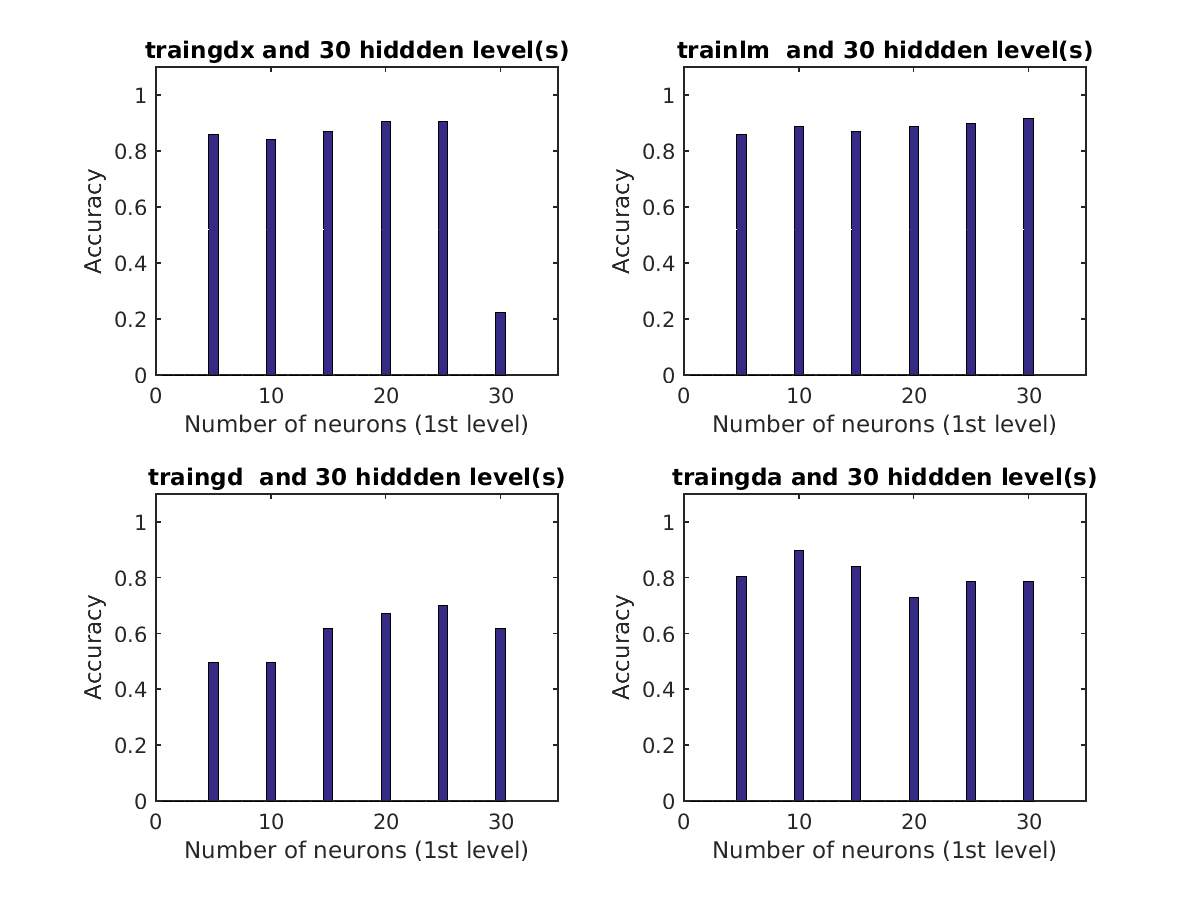
\includegraphics[width=0.8\textwidth]{fakelos/NNlvls-30.png}
			\caption{Απόδοση με 30 νευρώνες στο 2ο κρυφό επίπεδο} 	  
			\label{fig:2.NN-lvls30}
		\end{figure}
		
\section*{Ερώτημα 3 - Συνάρτηση ενεργοποίησης}
Στο ερώτημα αυτό συγκρίθηκε η απόδοση για 4 διαφορετικές συναρτήσεις ενεργοποίησης. Η purelin είναι απλώς μια γραμμική συνάρτηση, η tansig είναι συνάρτηση σιγμοειδούς υπερβολικής εφαπτομένης, η logsig λογαριθμική σιγμοειδής και η hardlim είναι hard limit. Οι γραφικές τους παραστάσεις φαίνονται στην εικόνα \ref{fig:3.Act-funcs} και τα αποτελέσματα για το accuracy στην εικόνα \ref{fig:3.Act-func-acc}. Αρχικά παρατηρούμε ότι οι hardlim και logsig έχουν τη χειρότερη απόδοση από τις 4, κάτι που είναι λογικό καθώς τα δεδομένα μας έχουν μέση τιμή 0 αλλά οι δύο αυτές συναρτήσεις έχουν πεδίο τιμών το $[0,1]$. Η συνάρτηση που κάνει τις γραφικές για τις διαφορετικές περιπτώσεις ειναι η \textit{plotActFunc.m}.

\begin{figure}[H]
	 		\centering
			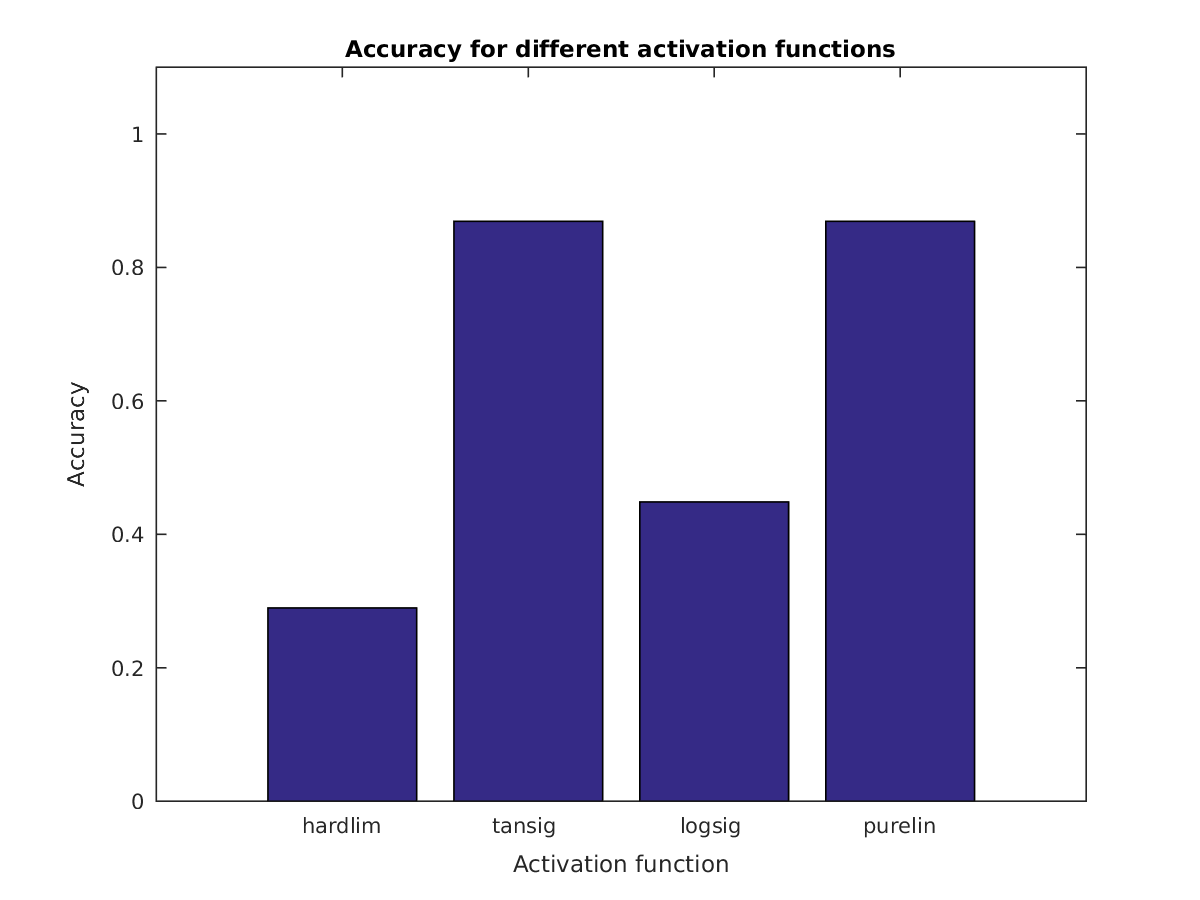
\includegraphics[width=0.7\textwidth]{fakelos/6a.actFunc-lvl1-30-lvl2-0.png}
			\caption{Αποδόση για διαφορετικες συναρτησεις ενεργοποίησης} 	  
			\label{fig:3.Act-func-acc}
		\end{figure}

\begin{figure}[H]
	 		\centering
			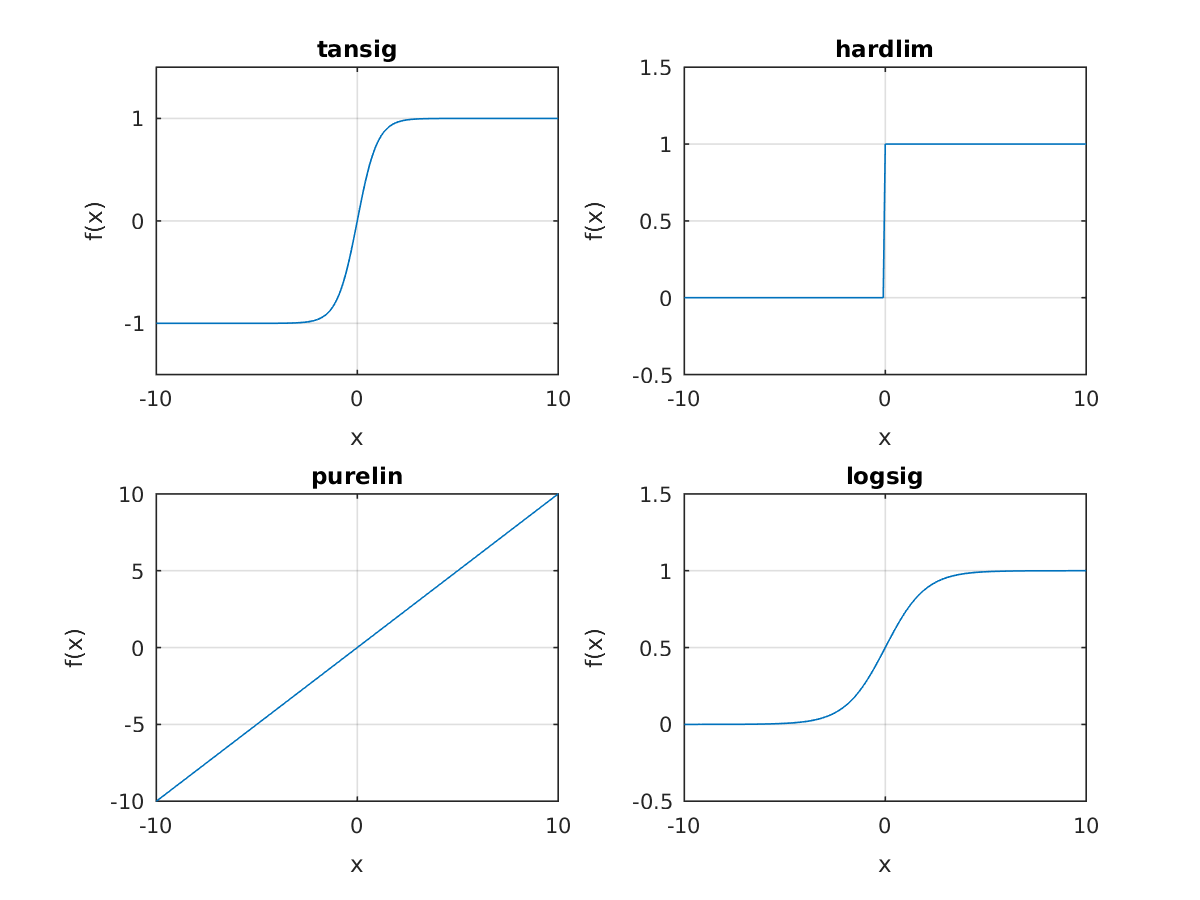
\includegraphics[width=0.7\textwidth]{fakelos/actFuncs.png}
			\caption{Οι συναρτήσεις ενεργοποίησης} 	  
			\label{fig:3.Act-funcs}
		\end{figure}
				
		
		
		
\section*{Ερώτημα 4 - Αλγορίθμος μάθησης}
Συγκρίθηκαν οι αλγόριθμοι μάθησης learngd και learngdm. Ο πρώτος αποτελεί την κλασσική υλοποίηση του backpropagation και υπολογίζει το correction στα βάρη ως εξής: 

\begin{equation}
\Delta w_{ij}(n)=\eta \delta_{j}(n)y_i(n)
\end{equation}

όπου $\eta$ είναι η παράμετρος μάθησης και  $\delta_{j}$ είναι το local gradient, και $y_i(n)$ η είσοδος. Στην περίπτωση του learngdm έχουμε έναν επιπλέον όρο ορμής, οπότε το correction θα είναι:

\begin{equation}
\Delta w_{ij}(n)=\alpha \Delta w_{ij}(n-1) + (1-\alpha)\eta \delta_{j}(n)y_i(n)
\end{equation}

 όπου το $\alpha$ είναι η σταθερά ορμής. \\
 Στην συνάρτηση learngd υπάρχει πρόβλημα όταν μειωθεί πολύ η παράμετρος μάθησης καθώς ενώ θα έχουμε ομαλές μεταβάσεις στον χώρο των βαρών, λόγω του ότι τα βάρη θα αυξάνονται με αργό ρυθμό, ο ρυθμός μάθησης θα είναι αργός. Αντίθετως, όταν ο ρυθμός αυξηθεί πολύ, οι αλλαγές στα βάρη θα είναι πολύ απότομες και υπάρχει περίπτωση να γίνεται "ταλάντωση" γύρω απο το σημείο που θέλουμε να φτάσουμε και να έχουμε ένα ασταθές δίκτυο. Η learngdm δεν αφήνει τόσο απότομες αλλαγες, και "μετριάζει" την ταλάντωση. Αυτό έχει ως αποτέλεσμα να συγκλίνει πιο αργά αλλά να φτάνει στο επιθυμητο αποτέλεσμα με καλύτερη ακρίβεια σε αντίθεση με την learngd που είναι αρκετά πιο γρήγορη. Στο δικό μας δίκτυο, η learngd είναι οριακά καλύτερη, αλλά λόγω όσων αναφέρθηκαν παραπάνω, θα χρησιμοποιούσαμε την learngdm. Το αποτέλεσμα στο accuracy φαίνεται στην εικόνα \ref{fig:4.Learn-algo}. 

\begin{figure}[H]
	 		\centering
			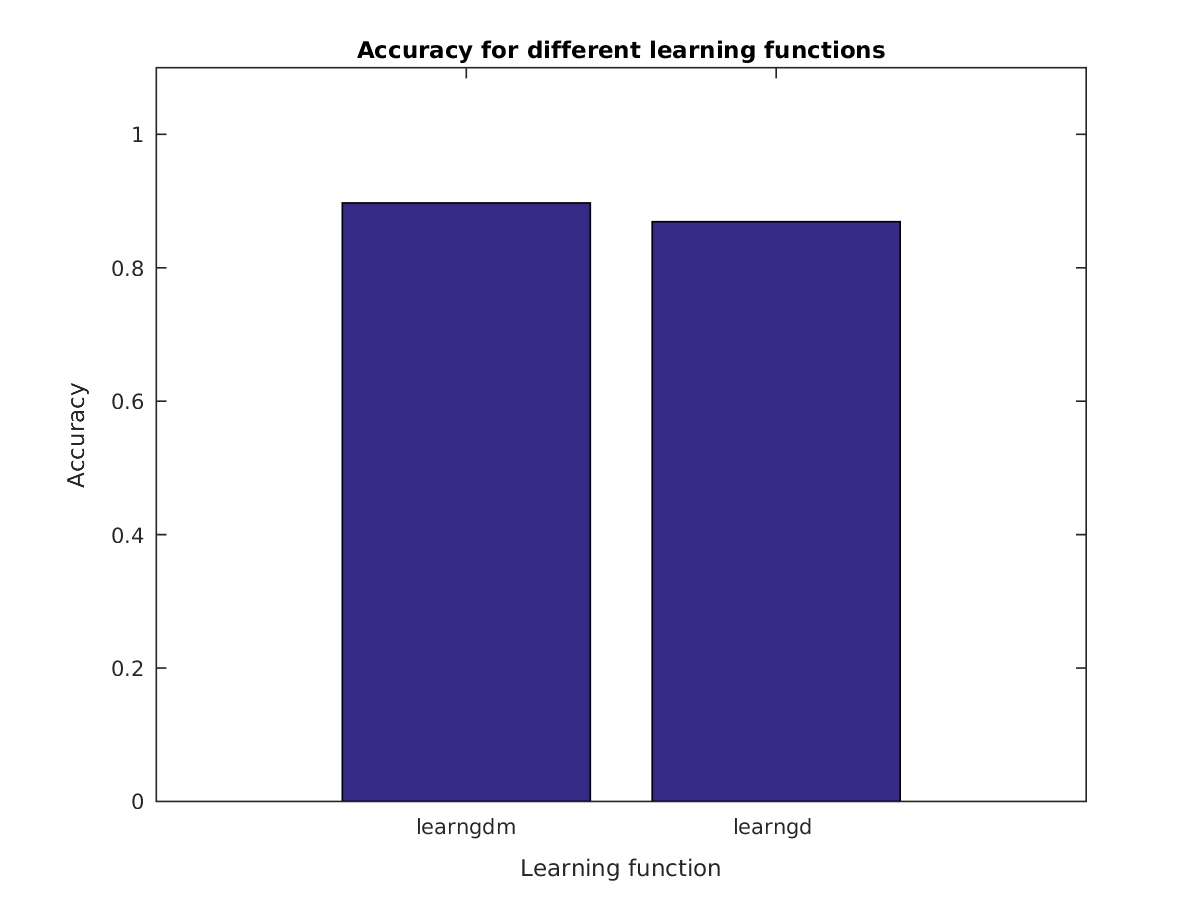
\includegraphics[width=0.8\textwidth]{fakelos/6b.learnFunc-lvl1-30-lvl2-0.png}
			\caption{Αποδόση για διαφορετικούς αλγορίθμους μάθησης}
			\label{fig:4.Learn-algo}
		\end{figure}
Η συνάρτηση για το συγκεκριμένο ερώτημα είναι η \textit{plotLearnFunc.m}. Το τρέξαμε για τις default (1000) εποχές.
		
\section*{Ερώτημα 5 - Early Stopping}
Σε αυτό το ερώτημα εξετάζεται η απόδοση του νευρωνικού με validation set και χωρίς αυτό. Η τεχνική του early stopping  λειτουργεί ως εξής: τα δεδομένα εκπαίδευσης χωρίζονται σε 2 ομάδες, μια ομάδα με δεδομένα εκπαίδευσης και τα υπόλοιπα είναι το validation set. Κατα τη διάρκεια της εκπαίδευσης του δικτύου (χρησιμοποιώντας μόνο την πρώτη ομάδα δεδομένων), ελέγχεται συνεχώς το σφάλμα στη δευτερη ομάδα. Τυπικά, το σφάλμα στο validation set στην αρχή θα μειώνεται καθώς το δίκτυο εκπαιδεύεται, αλλά κάποια στιγμή θα φτάσει σε ένα minimum και θα αρχίσει να αυξάνεται πάλι. Αν συνεχίσει να αυξάνει για συγκεκριμένο αριθμό επαναλήψεων, η εκπαίδευση σταματάει, για να αποφευχθεί το overfitting, και επιστρέφονται τα βάρη που είχαν βρεθεί για το minimum του σφάλματος. 

Στα μέχρι τώρα ερωτήματα, το 20\% χρησιμοποιούνταν ως validation set. Στη δική μας περίπτωση βλέπουμε ότι με validation set σταματήσαμε στις 7 εποχές, ενώ τελικά το accuracy του δικτύου ήταν αρκετα καλύτερο. Παρατηρούμε επίσης ότι δε σταματάει αμέσως μόλις το σφάλμα στο Validation set γίνει πιο μεγάλο, καθώς μπορεί να είναι ενα τοπικό μέγιστο και να συνεχίσει να πέφτει μετά (όπως στην εικόνα \ref{fig:5.error-with-vs}), ενώ ακριβώς επειδή σταματάει νωρίτερα, η μέθοδος αυτή θα είναι συνήθως αρκετά γρηγορότερη απο το να μην χρησιμοποιούσαμε validation set, όπου και θα έπρεπε να κάνει (εδω) 1000 εποχές για την πλήρη εκπαίδευση.

\begin{figure}[H]
	 		\centering
			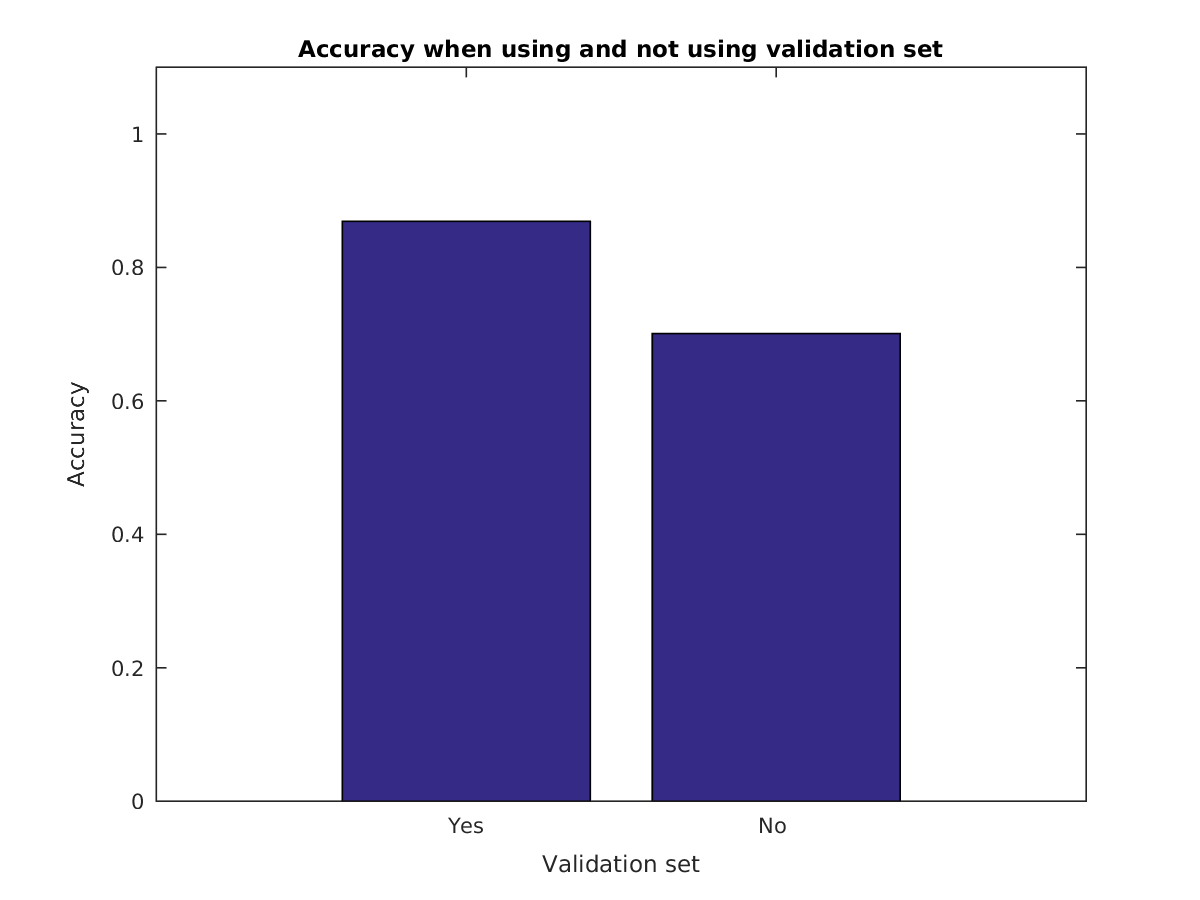
\includegraphics[width=0.7\textwidth]{fakelos/6c.valSet-lvl1-30-lvl2-0.png}
			\caption{Αποδόση με και χωρίς validation set}
			\label{fig:5.Val-set1}
		\end{figure}

\begin{figure}[H]
	 		\centering
			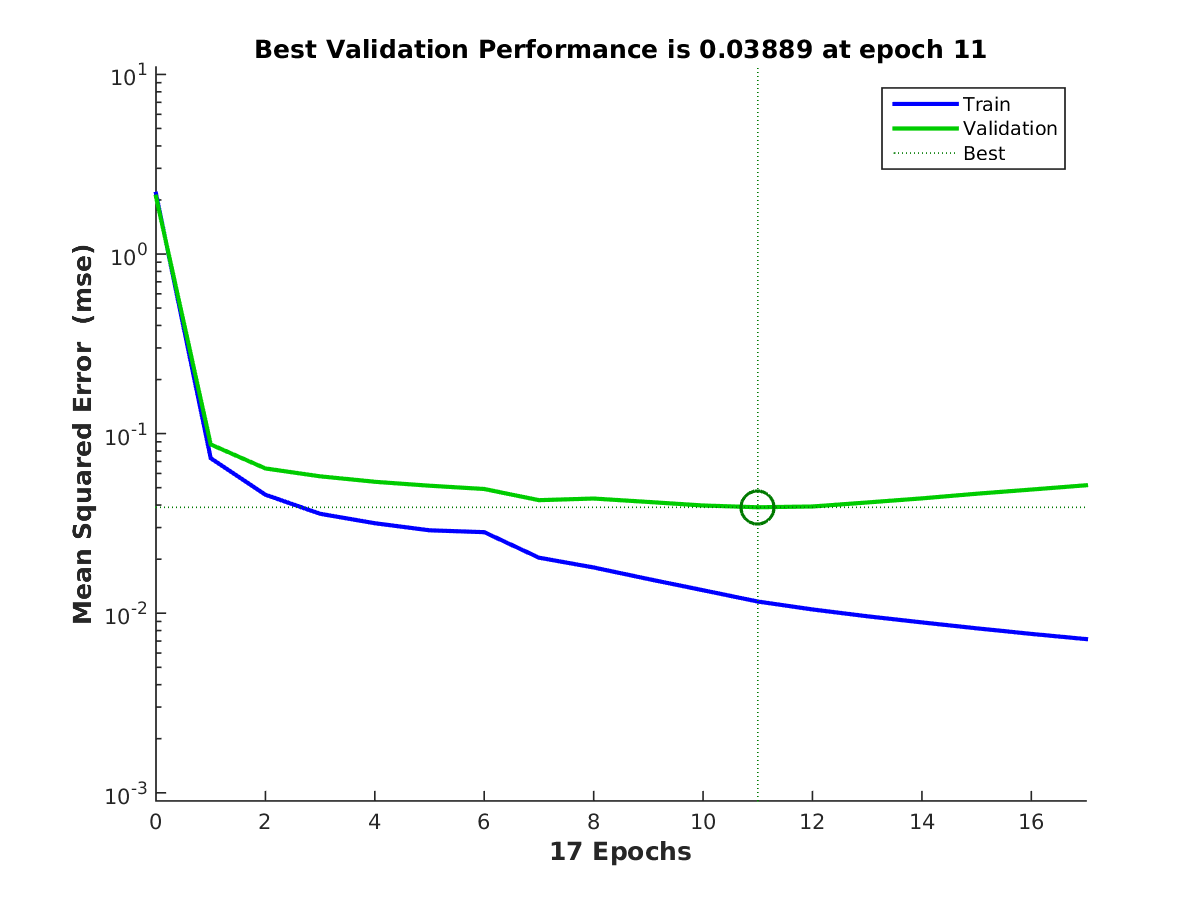
\includegraphics[width=0.7\textwidth]{fakelos/6c.perf1-lvl1-30-lvl2-0.png}
			\caption{Μέσο σφάλμα με validation set}
			\label{fig:5.error-with-vs}
		\end{figure}
		
\begin{figure}[H]
	 		\centering
			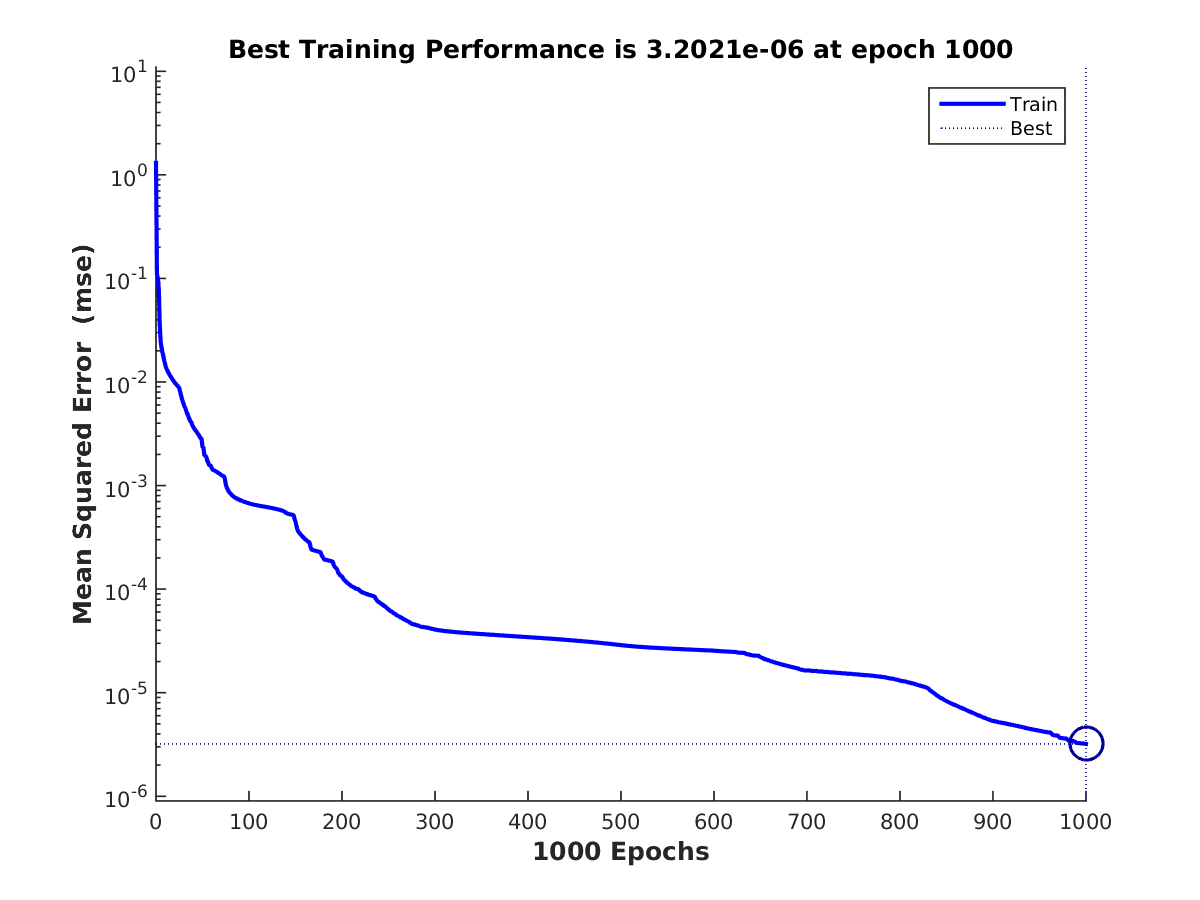
\includegraphics[width=0.7\textwidth]{fakelos/6c.perf2-lvl1-30-lvl2-0.png}
			\caption{Μέσο σφάλμα χωρίς validation set}
			\label{fig:5.error-without-vs}
		\end{figure}
		
		Ο κώδικας για την παραγωγή των γραφικών του ερωτήματος είναι στο \textit{plotValSet.m}.
\section*{Ερώτημα 6 - Αριθμός εποχών}
Σε αυτό το ερώτημα θα προσπαθήσουμε να εκτιμήσουμε το πως επιδρά το διαφορετικό πλήθος εποχών στην απόδοση. Παίρνουμε τιμές σε ένα εύρος 5 γύρω από την τιμή που βρήκαμε στο προηγούμενο ερώτημα. Περιμένουμε καλύτερη απόδοση όσο το πλήθος των εποχών παραμένει κοντά στην επικρατέστερη τιμή που ήταν το 7. Παρ' όλα αυτά λόγω των αποκλίσεων των αποτελεσμάτων ανά εκτέλεση, περιμένουμε διαφοροποιήσεις. Επίσης λόγω της μικρής τιμής για το καλύτερο πλήθος εποχών εκπαίδευσης έχουμε αναγκαστικά και μικρό εύρος στο οποίο αναζητάμε τώρα διαφοροποιήσεις. Σ' αυτό το ερώτημα κριτήριο τερματισμού δεν υπήρχε και κάθε κύκλος εκπαίδευσης ολοκληρωνόταν έπειτα από το συγκεκριμένο αριθμό εποχών. Παραθέτουμε έπειτα το διάγραμμα Accuracy συναρτήσει του αριθμού των εποχών.
\begin{figure}[H]
	 		\centering
			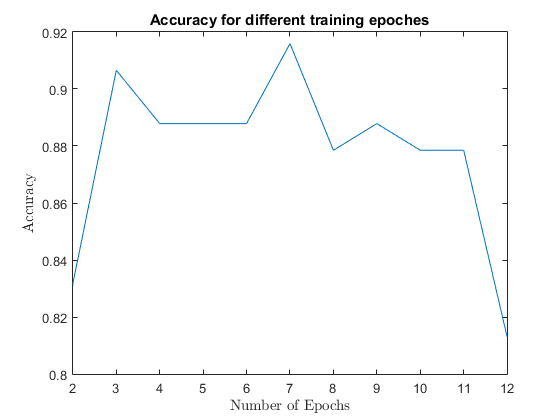
\includegraphics[width=0.8\textwidth]{fakelos/6d-7epochRange.png}
			\caption{ Accuracy συναρτήσει του αριθμού εποχών}
			\label{fig:6.epochs}
		\end{figure}
		
Πράγματι το παραπάνω διάγραμμα ακολουθεί την προσδοκόμενη συμπεριφορά. Η συνάρτηση για το συγκεκριμένο ερώτημα είναι η \textit{epochRange.m}.

\section*{Ερώτημα 7 - Ρυθμός μάθησης}
Μεγάλοι ρυθμοί μάθησης μπορεί να οδηγήσουν σε μη σωστή εκπαίδευση καθώς είναι πιθανό να αγνοηθούν τοπικά ελάχιστα είτε να παρατηρήσουμε 'ταλαντώσεις'. Απ' την άλλη όμως επιτυγχάνουμε καλύτερη ταχύτητα εκπαίδευσης. Ο μικρός ρυθμός αποτελεί πρόβλημα όταν είναι εξαιρετικά χαμηλός οπότε και παρατηρούνται φαινόμενα υπερεκπαίδευσης. 
\begin{figure}[H]
	 		\centering
			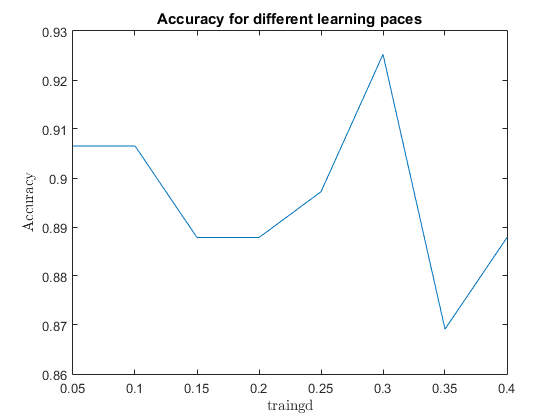
\includegraphics[width=0.8\textwidth]{fakelos/6e-first.png}
			%\caption{Αποδόση για διαφορετικούς αλγορίθμους μάθησης}
			\label{fig:7.learn-rate1}
		\end{figure}
		
\begin{figure}[H]
	 		\centering
			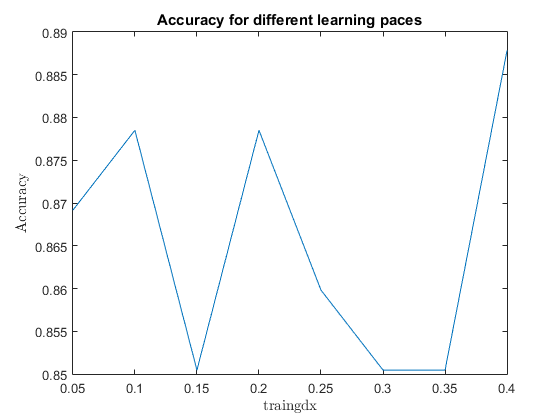
\includegraphics[width=0.8\textwidth]{fakelos/6e-second.png}
			\caption{Αποδόση για διαφορετικούς αλγορίθμους μάθησης}
			\label{fig:7.learn-rate2}
		\end{figure}		
		
Η traingd όπως και αναμενόταν δεν επηρεάζεται ουσιαστικά από την αλλαγή του ρυθμού μάθησης αφού δεν διαθέτει και όρο ορμής. Αντίθετα η traingdx φαίνεται να παρουσιάζει ασταθή συμπεριφορά ως προς αυτή την παράμετρο. Τέλος η απόδοση της traingd για τους διάφρορους ρυθμούς μάθησης είναι συνολικά μεγαλύτερη από αυτή της traingdx, συνεπώς μεταξύ των δύο θα επιλέγαμε την traingd. Για το συγκεκριμένο ερώτημα ο κώδικας βρίσκεται στο αρχείο \textit{stepLearning.m}. Η εκπαίδευση του δικτύου έγινε για 30 χιλιάδες εποχές.

\section*{Ερώτημα 8- Απόδοση ανά κατηγορία }
Είναι γεγονός πως παρατηρούμε αποκλίσεις μεταξύ των αποδόσεων, διαφορετικών κατηγοριών. Πιθανότατα οι συγκεκριμένες αποκλίσεις έχουν να κάνουν με το γεγονός ότι διαφορετικές κατηγορίες παρουσιάζουν και διαφορετική δυσκολία στην αναγνώριση τους. Ένας παράγοντας μπορεί να είναι ομοιότητες που παρουσιάζουν μεταξύ τους οι εικόνες δύο κατηγοριών. Ένας τρόπος αντιμετώπισης αυτού του γεγονότος θα ήταν η υπεραντιπροσώπευση αυτών των κατηγοριών στο δείγμα εκπαίδευσης με στόχο την καλύτερη αποσαφήνιση των μεταξύ τους διαφορών. 

\begin{figure}[H]
	 		\centering
			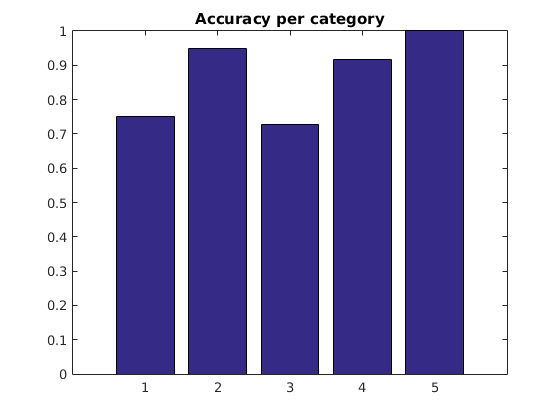
\includegraphics[width=0.8\textwidth]{fakelos/acc_per_cat.png}
			\caption{Αποδόση για κάθε κατηγορία}
			\label{fig:8.acc-per-cat}
		\end{figure}	
		
		
\section*{Επιμύθιο }
Συγκεντρωτικά με βάση τα συμπεράσματα των παραπάνω διερευνήσεων είμαστε πλέον σε θέση να προσδιορίσουμε τις κατάλληλες παραμέτρους για την βέλτιστη λειτουργία του νευρωνικού μας δικτύου. Επιλέξαμε ένα επίπεδο με 30 Νευρώνες, καλύτερη συνάρτηση εκπαίδευσης προέκυψε η trainglm, ενώ για συνάρτηση ενεργοποίησης επιλέξαμε την tansing. Ο αλγόριθμος μάθησης που θα χρησιμοποιήσουμε είναι ο learngd και τέλος θα κάνουμε χρήση του validation set. Παραθέτουμε στη συνέχεια την αποδοτικότητα της συγκεκριμένης υλοποίησης.
\begin{figure}[H]
	 		\centering
			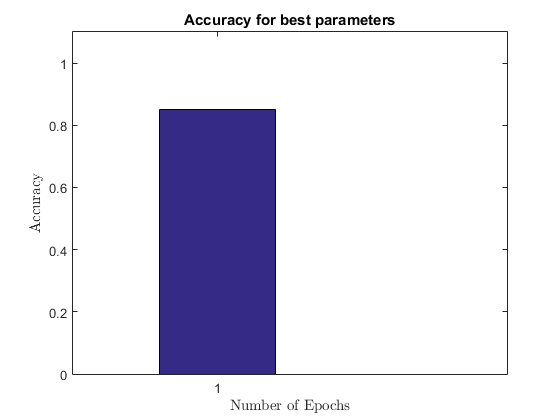
\includegraphics[width=0.8\textwidth]{fakelos/step7.png}
			\caption{Αποδόση Νευρωνικού Δικτύου με βέλτιστες παραμέτρους}
			\label{fig:4.Learn-algo}
		\end{figure}

Για το συγκεκριμένο ερώτημα ο κώδικας βρίσκεται στο αρχείο \textit{bob.m}. 
				
\section*{Η μέθοδος της αποσύνθεσης βαρών }
Σκοπός μας με την μέθοδο της αποσύνθεσης των βαρών είναι να εξαλείψουμε βάρη του δικτύου που δεν υπερβαίνουν ένα όριο καθώς λειτουργούν περισσότερο ως θόρυβος. Για το σκοπό αυτό τρέξαμε τον τροποποιημένο αλγόριθμο που μας δόθηκε με διάφορες τιμές για την τιμή του λ,και του κατωφλίου d. Τελικά επιλέξαμε λ=0.15 και d=0.02  
\begin{figure}[H]
	 		\centering
			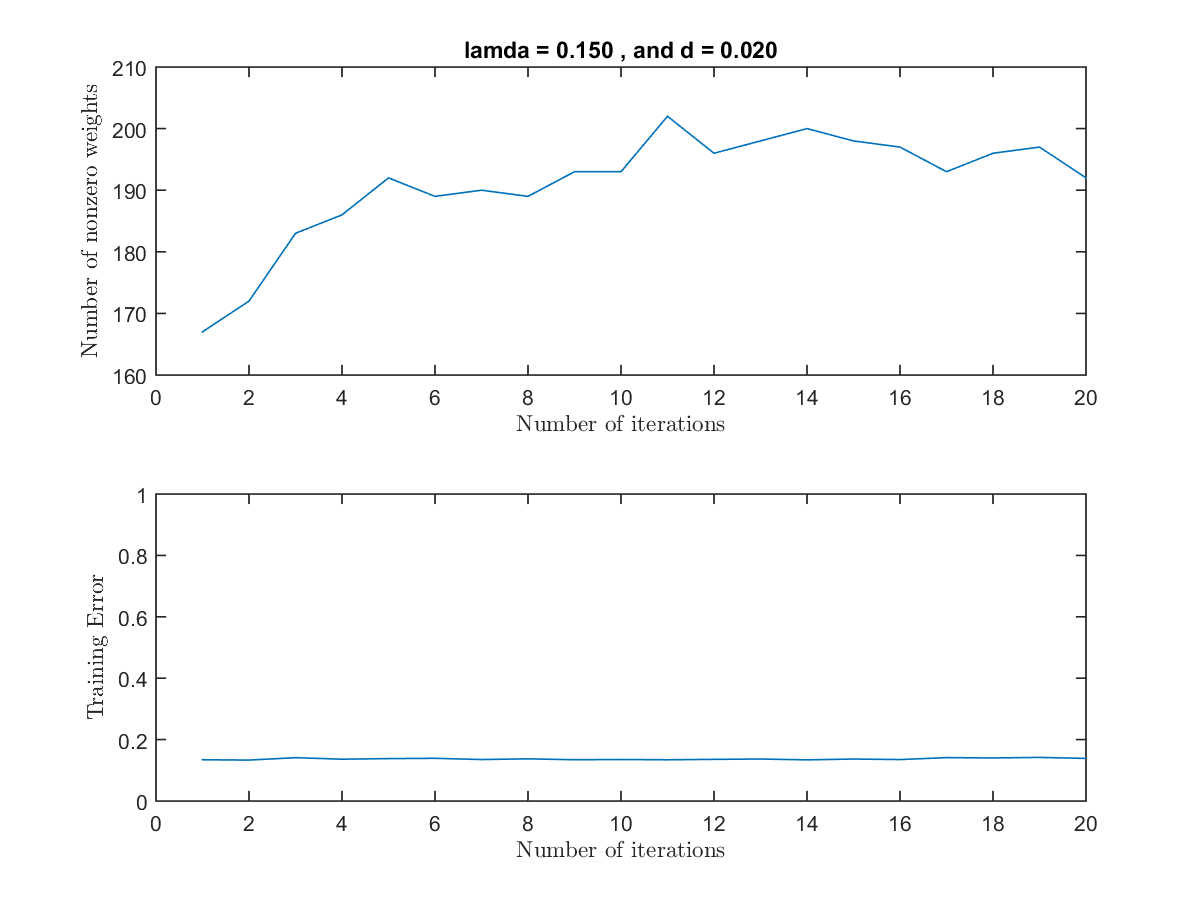
\includegraphics[width=0.8\textwidth]{fakelos/weight4.png}
			\caption{Μη μηδενικά βάρη και μέσο τετραγωνικό σφάλμα - εκπαίδευση με weight decay }
			\label{fig:4.Learn-algo}
		\end{figure}		
		
Η μέθοδος της αποσύνθεσης των βαρών υλοποιήθηκε στο αρχείο  \textit{weightDecay.m}. 	

%\section{Κώδικας}
%\subsection{Main}
%\label{subsec:main}
%\lstinputlisting[language=Matlab]{code/mainTotal.m}	

%\subsection{Preprocessing}
%\label{subsec:preproc}
%\lstinputlisting[language=Matlab]{code/preproc.m}	

%\subsection{Συνάρτηση myTrain}
%\label{subsec:myTrain}
%\lstinputlisting[language=Matlab]{code/myTrain.m}		

%\subsection{Plots για Learning function}
%\label{subsec:learnFunc}
%\lstinputlisting[language=Matlab]{code/plotLearnFunc.m}

%\subsection{Plots για Early Stopping}
%\label{subsec:earlStop}
%\lstinputlisting[language=Matlab]{code/plotValSet.m}

%\subsection{Plots για αριθμό εποχών}
%\label{subsec:earlStop}
%\lstinputlisting[language=Matlab]{code/epochRange.m}

%\subsection{Plots για learning rate}
%\label{subsec:earlStop}
%\lstinputlisting[language=Matlab]{code/stepLearning.m}

\end{document}
